Im Folgenden sind die während des Versuchs aufgenommenen Daten und die aus diesen
berechneten Größen tabellarisch aufgetragen. An entsprechender Stelle sind Erklärungen
zu den Werten und Berechnungen gegeben.\\

In \autoref*{tab:Daten} befinden sich die für die Auswertung verwendeten Messdaten für die Temperaturen
$T_{1}\ \text{und}\ T_{2}$, die Drücke $p_{b}\ \text{und}\ p_{a}$, sowie die Zeit $t$ der Aufnahme nach Beginn des Versuchs.

\begin{table}[!h]
\centering
\begin{tabular}{|r|C|C|C|C|}
	\hline
	         Zeit & {Temperatur}       & {Druck}             & {Temperatur}       & {Druck}             \\
	$t\,[\si{s}]$ & $T_{1}\,[\si{°C}]$ & $p_{b}\,[\si{bar}]$ & $T_{2}\,[\si{°C}]$ & $p_{a}\,[\si{bar}]$ \\ \hline\hline
	            0 & \num{26,6(1)}      & \num{7,0(5)}        & \num{17,4(1)}      & \num{4,6(2)}        \\
	           90 & \num{28,0(1)}      & \num{7,5(5)}        & \num{16,5(1)}      & \num{4,6(2)}        \\
	          180 & \num{30,1(1)}      & \num{7,9(5)}        & \num{15,1(1)}      & \num{4,4(2)}        \\
	          270 & \num{32,1(1)}      & \num{8,0(5)}        & \num{13,9(1)}      & \num{4,2(2)}        \\
	          360 & \num{34,0(1)}      & \num{8,5(5)}        & \num{12,7(1)}      & \num{4,1(2)}        \\
	          450 & \num{35,2(1)}      & \num{9,0(5)}        & \num{11,9(1)}      & \num{4,0(2)}        \\
	          540 & \num{37,0(1)}      & \num{9,0(5)}        & \num{10,9(1)}      & \num{4,0(2)}        \\
	          630 & \num{38,6(1)}      & \num{9,5(5)}        & \num{9,8(1)}       & \num{3,9(2)}        \\
	          720 & \num{40,2(1)}      & \num{10,0(5)}       & \num{8,9(1)}       & \num{3,9(2)}        \\
	          810 & \num{41,7(1)}      & \num{10,0(5)}       & \num{8,0(1)}       & \num{3,8(2)}        \\
	          900 & \num{43,1(1)}      & \num{10,5(5)}       & \num{7,2(1)}       & \num{3,6(2)}        \\
	          990 & \num{44,5(1)}      & \num{11,0(5)}       & \num{6,5(1)}       & \num{3,6(2)}        \\
	         1080 & \num{45,8(1)}      & \num{11,0(5)}       & \num{5,9(1)}       & \num{3,6(2)}        \\
	         1170 & \num{46,6(1)}      & \num{11,5(5)}       & \num{5,4(1)}       & \num{3,6(2)}        \\
	         1260 & \num{47,9(1)}      & \num{12,0(5)}       & \num{4,9(1)}       & \num{3,6(2)}        \\
	         1350 & \num{49,0(1)}      & \num{12,0(5)}       & \num{4,4(1)}       & \num{3,5(2)}        \\ \hline
\end{tabular}
\caption{Messwerte der Temperaturen und Drücke}
\label{tab:Daten}
\end{table}

In \autoref{fig:T1} und \ref{fig:T2} sind die Temperaturverläufe für $T_{1}$ und $T_{2}$ jeweils mit der entsprechenden 
Regressionskurve dargestellt.
Die mit Hilfe der Python Bibliothek \emph{SciPy} \cite{SciPy} bestimmten Regressionsparameter für die Kurven der Form
$T(t) = At^{2} + Bt + C$ sind in \autoref{tab:param} gelistet.\\

\begin{table}[!h]
  	\centering
  
   	\begin{tabular}{|c||c|c|c|}
   		\hline
   		Funktion & $A\,[\si{\kelvin\per\second\squared}]$ & $B\,[\si{\kelvin\per\second}]$& $C\,[\si{\kelvin}]$\\ \hline \hline
   		$T_{1}$& \num{-3.87(29)e-06}& \num{2.20(4)e-04}& \num{299.49(12)}\\
    		$T_{2}$& \num{3.59(20)e-06}& \num{-1.47(3)e-02}& \num{290.76(9)}\\
    		\hline
   	\end{tabular}
   	\caption{Parameter der Regression mit $T(t) = At^{2} + Bt + C$ \label{tab:param}}
\end{table}
	
\begin{figure}[!h]
	\centering
	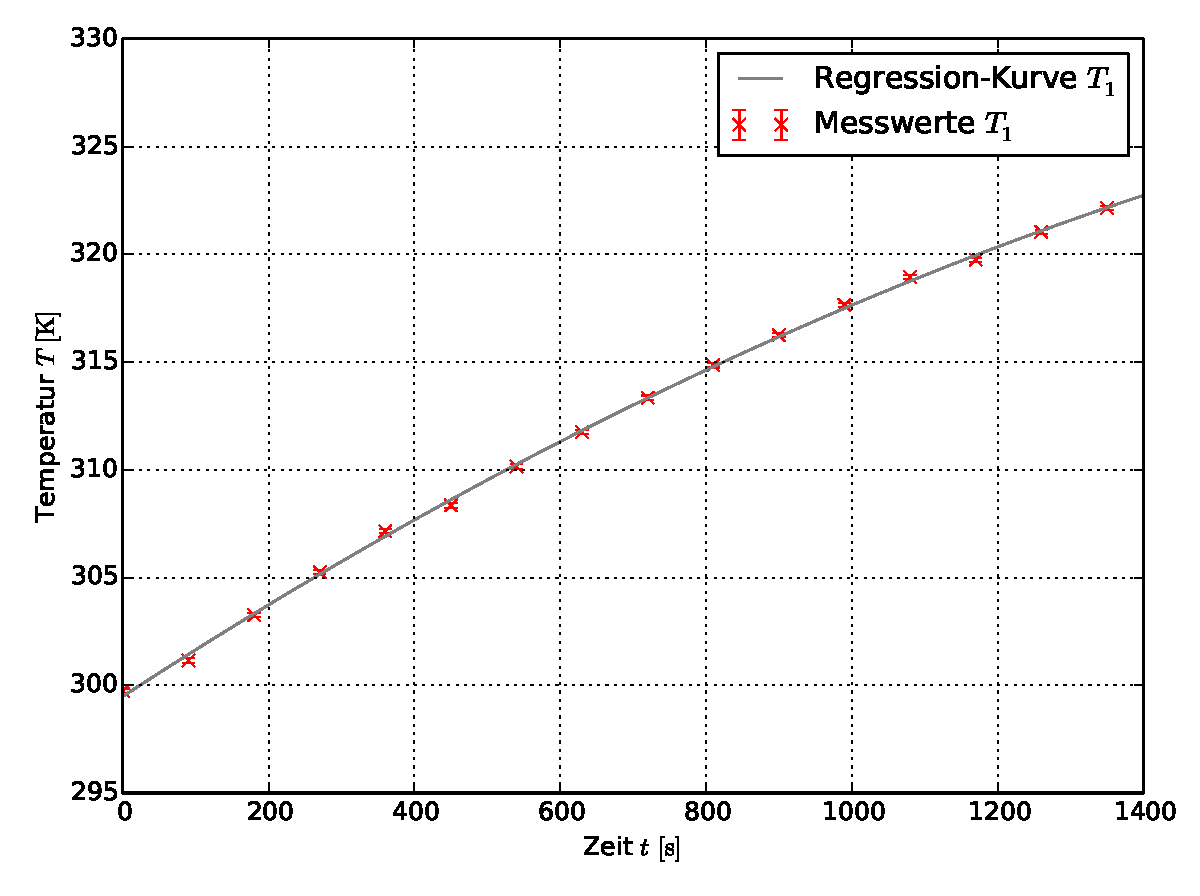
\includegraphics[scale=0.62]{Plots/Temperaturverlauf_T1.pdf}
 	\caption{Temperaturverlauf mit Regressionskurve von $T_{1}$}
 	\label{fig:T1}
\end{figure}

\begin{figure}[!h]
	\centering
	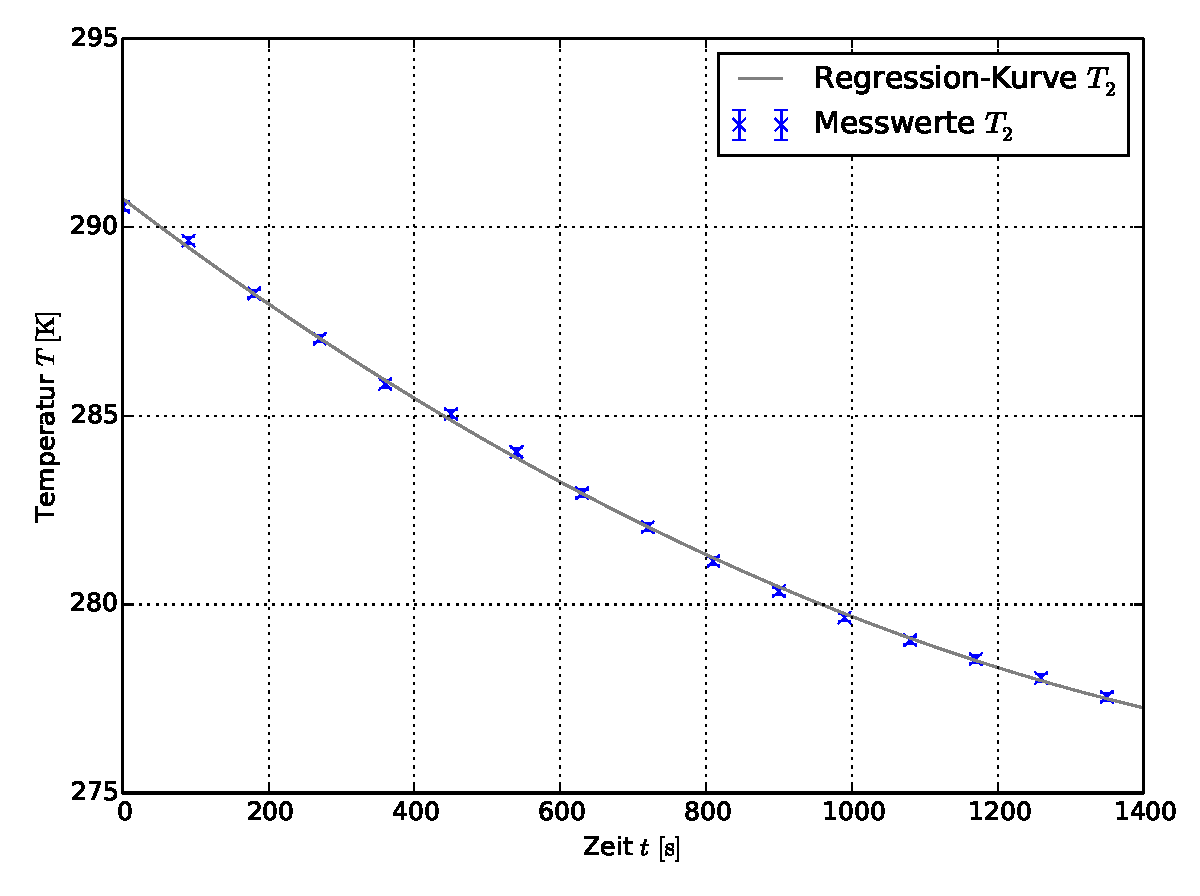
\includegraphics[scale=0.62]{Plots/Temperaturverlauf_T2.pdf}
	\caption{Temperaturverlauf mit Regressionskurve von $T_{2}$}
	\label{fig:T2}
\end{figure}
\newpage
Aus den Regressionskurven für die Temperaturverläufe lassen sich nun deren Differentialquotienten 
$\od{T_{1}}{t}$ und $\tod{T_{2}}{t}$
bestimmen, durch die, die gesuchten Apparaturgrößen berechnet werden können. Die Differenzialquotienten $\od{T_{1}}{t}$ und die 
berechneten, idealen und realen, Güteziffern sowie deren Verhältnis sind in \autoref{tab:Güte} und die 
Differenzialquotienten $\od{T_{2}}{t}$ und der daraus bestimmte Massendurchsatz des Transportgases $\od{m}{t}$
in \autoref{tab:Masse} zu finden. Die angegebenen Fehler wurde dabei, durch die jeweils referenzierte Gleichung (römische Nummerierung)
berechnet, die in \autoref{sec:Fehlerrechnung} zu finden ist.

	\subsection{Güteziffern}
Die Berechnung der idealen Güteziffer erfolgt nach \eqref{eq:vid} durch einsetzen der Temperaturen $T_{1}$ und $T_{2}$ zu den entsprechenden
Zeiten. 	
Die reale Güteziffer errechnet sich aus durch Einsetzen von \eqref{eq:dQ1} in \eqref{eq:vreal} und Ersetzen des Differenzenquotienten
$\tfrac{\Delta T_{1}}{\Delta t}$ durch den Differentialquotienten $\od{T_{1}}{t}$ sodass man 

\begin{empheq}{equation}
	\nu_{real} = \dfrac{(m_{1}c_{w} + m_{k}c_{k})}{P} \dod{T_{1}}{t} 
	\label{eq:vreal2}
\end{empheq}
erhält. Dabei ist $m_{1}c_{w}$ die Wärmekapazität des Wassers in Reservoir 1, die sich aus dem Produkt der Masse $m_{1}$ und der spezifischen Wärmekapazität $c_{w}$ des Wassers ergibt.
Mit $c_{w} = \SI{4.182}{kJkg^{-1}K^{-1}}$ \cite{Kuchling07} und $m_{1} = V_{1}\rho_{w} = \SI{3.992}{kg}$, wobei $V_{1} = \SI{4}{dm^{3}}$ das Volumen und $\rho_{w} = \SI{0.998}{gcm^{-3}}$ 
die Dichte des Wassers bei $\SI{21}{°C}$ \cite{Kuchling07} sind. Die Wärmekapazität der Apparatur ist gegeben durch $m_{k}c_{k} = \SI{750}{JK^{-1}}$ und die gemessene Leistung ist $P = \SI{125(5)}{W}$.\\

\begin{table}[!h]
	\centering
	\begin{tabular}{|c|c|c|c|c|}
		\hline
		    Zeit      &    Differentialquotient    & reale Güteziffer  & ideale Güteziffer &     relativer Unterschied     \\
		$t\,[\si{s}]$ & $\od{T_{1}}{t}\,[Ks^{-1}]$ & $\nu_{real}\,\eqref{eq:Err_vreal}$ &  $\nu_{id}\,\eqref{eq:Err_vid}$ & $\frac{\nu_{real}}{\nu_{id}}$ \\ \hline\hline
		     270      &        \num{0.0206(4)}         & \num{2.9(1)}  & \num{20.2(2)} &          \num{0.142}          \\
		     450      &        \num{0.0192(5)}         & \num{2.7(1)}  & \num{14.42(09)} &          \num{0.186}          \\
		     630      &        \num{0.0178(5)}         & \num{2.5(1)}  & \num{11.88(06)} &          \num{0.210}          \\
		     810      &        \num{0.0165(6)}         & \num{2.30(09)}  & \num{10.01(04)} &          \num{0.229}          \\ \hline
	\end{tabular}
	\caption{Reale und ideale Güteziffer im Verhältnis}
	\label{tab:Güte}
\end{table} 

	\subsection{Massendurchsatz und mechanische Leistung}
Die Berechnung des Massendurchsatzes $\od{m}{t}$ erfolgt durch Einsetzen von \eqref{eq:dQ2} in \eqref{eq:dM} (mit Differentialquotienten), wodurch man die Gleichung 

\begin{empheq}{equation}
(m_{2}c_{w} + m_{k}c_{k})\dod{T_{2}}{t} = L \dod{m}{t}
\label{eq:dm2}
\end{empheq}
erhält.

Zur Bestimmung der Verdampfungswärme $L$ wurden in \autoref{fig:pT} die Messwerte für $ p_{b} $ halb-logarithmisch gegen die reziproken Temperaturen $\tfrac{1}{T_{1}}$ auf getragen. 
Aus \cite{V203} kann entnommen werden das zwischen $p$ und $T$ der exponentielle Zusammenhang

\begin{empheq}{equation}
 	p(T) = p_{0}\exp(\dfrac{-L}{RT})   
	\label{eq:pTexp}
\end{empheq}
besteht. Durch die halb-logarithmische Skalierung und dem Aufragen gegen den Kehrwert der Temperatur  $ x := \tfrac{1}{T_{1}}$  erhält man daraus eine Geradengleichung der Form

\begin{empheq}{equation}
 	\ln(p(x)) = \dfrac{-L}{R}x + \ln(p_{0}) .
	\label{eq:pTlin}
\end{empheq}

\begin{figure}[!h]
	\centering
	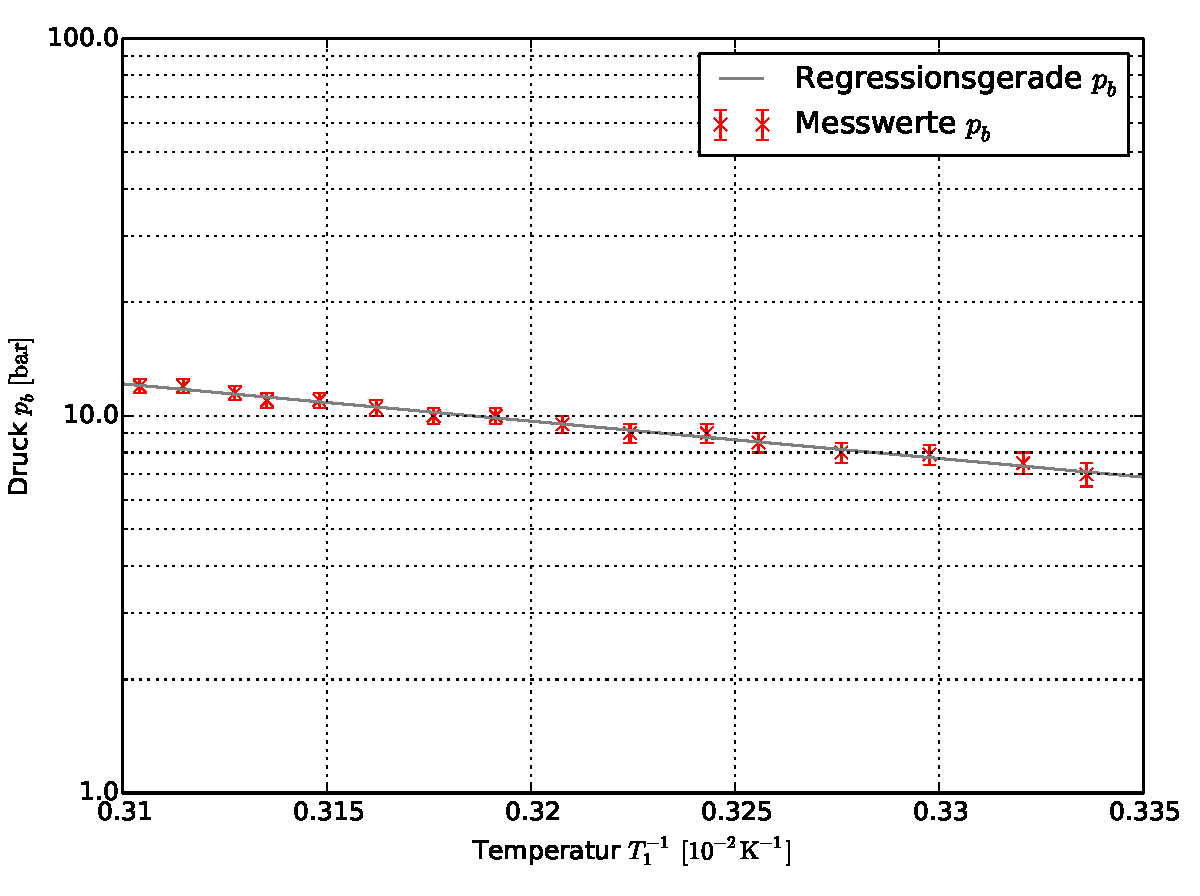
\includegraphics[scale = 0.75]{Plots/Regression_pT.pdf}
	\caption{Regression der $(T_{1},p_{b})$ Wertepaare}
	\label{fig:pT}
\end{figure}

Durch die mit \emph{Scipy} \cite{SciPy} durchgeführte lineare Regression erhält man die Geradensteigung 
\[   
	\tfrac{-L}{R} = \SI{-2277(60)}{K} 
\] 
und daraus mit der allgemeinen Gaskonstante $R = \SI{8.315}{Jmol^{-1}K^{-1}}$\cite{SciPy} die Verdampfungswärme zu

\begin{empheq}{equation*}
 	L = \SI{1.89(5)e04}{Jmol^{-1}} 
\end{empheq}
wobei der angegebene Fehler mit \eqref{eq:Err_L} berechnet wurde. Durch Einsetzen dieses Wertes und der Werte $m_{2}c_{w} = \SI{16694,44}{JK^{-1}}$ und
 $m_{k}c_{k} = \SI{750}{JK^{-1}}$ in \eqref{eq:dm2} 
ergibt sich jeweils der gesuchte Massendurchsatz.\\

Bei Betrachtung der Einheiten
\begin{empheq}{align*}
	\si{Js^{-1}} &= \si{Jmol^{-1}} \cdot \left[ \od{m}{t}  \right] \\\Leftrightarrow\; \si{mols^{-1}} &= \left[ \od{m}{t}  \right]  
\end{empheq} 
ist festzustellen, dass sich dieser Massendurchsatz auf ein Mol des gesuchten Stoffes bezieht. Durch Multiplikation des erhaltenen Massendurchsatzes mit der molaren Masse von
Dichlordifluormethan $M_{\ce{Cl2F2C}} = \SI{120}{gmol^{-1}}$\footnote{Berechnet aus den molaren Massen der Komponenten \cite{Kuchling07}} erhält man den in \autoref{tab:Masse} aufgeführten
Massendurchsatz. 

Durch diesen kann unter Verwendung von \eqref{eq:Pmech} die mechanische Leistung des Kompressors bestimmt werden.
Das $\rho$ in \eqref{eq:Pmech} ist dabei durch die allgemeine Gasgleichung
\begin{empheq}{equation}
	pV = nRT
	\label{eq:Gas}
\end{empheq} 
den gegebenen Größen \cite{V206} des verwendeten Gases (\ce{Cl2F2C}), Dichte unter Normalbedingungen\footnote{ $T_{0} = \SI{0}{°C}$ und $p_{0} = \SI{1}{bar}$} 
$\rho_{0} = \SI{5.51}{gl^{-1}}$ und dem Adiabatenexponent $\kappa = \num{1.14}$ und den vorliegenden Zustandsgrößen $T_{2}$ und $p_{a}$ zu berechnen. 
Man erhält damit die Gleichung 
\begin{empheq}{equation}
	\rho = \dfrac{T_{2}p_{0}}{p_{a}T_{0}\rho_{0}}.
	\label{eq:Rho}
\end{empheq} 
Durch Einsetzen von \eqref{eq:Rho} in \eqref{eq:Pmech} erhält man
\begin{empheq}{equation}
	P_{mech} = \dfrac{1}{\kappa - 1}\left(p_{b}\sqrt[\kappa]{\dfrac{p_{a}}{p_{b}}} - p_{a} \right) \dfrac{p_{a}T_{0}\rho_{0}}{T_{2}p_{0}} \dod{m}{t}
	\label{eq:Pmech2}
\end{empheq}   
womit die gesuchte mechanische Leistung aus den gegebenen Größen berechnen kann.

\begin{table}[!h]
	\centering
	\begin{tabular}{|c|c|c|c|}
		\hline
		    Zeit      &    Differentialquotient    &       Massendurchsatz       & Mechanische Leistung \\
		$t\,[\si{s}]$ & $\od{T_{2}}{t}\,[Ks^{-1}]$\,\eqref{eq:Err_dT} & $\od{m}{t}\,[\si{gs^{-1}}]\,$\eqref{eq:Err_dm} & $P_{mech}\,[\si{W}]$ \\ \hline\hline
		     270      &      \num{-0.0134(2)}      &       \num{1.48(5)}       &     \num{15.075}     \\
		     450      &      \num{-0.0121(3)}      &       \num{1.37(5)}       &     \num{16.976}     \\
		     630      &      \num{-0.0108(3)}      &       \num{1.19(5)}       &     \num{16.843}     \\
		     810      &      \num{-0.0095(4)}      &       \num{1.05(5)}       &     \num{17.234}     \\ \hline
	\end{tabular}
	\caption{Massendurchsatz und mechanische Leistung des Transportgases}
	\label{tab:Masse}
\end{table}



 
		